\newif\ifshowsolutions
\showsolutionstrue
\documentclass{article}
\usepackage{listings}
\usepackage{amsmath}
\usepackage{subfig}
\usepackage{amsthm}
\usepackage{amsmath}
\usepackage{amssymb}
\usepackage{graphicx}
\usepackage{mdwlist}
\usepackage{geometry}
\usepackage{titlesec}
\usepackage{palatino}
\usepackage{mathrsfs}
\usepackage{fancyhdr}
\usepackage{paralist}
\usepackage{todonotes}
\usepackage{tikz}
\usepackage{float} % Place figures where you ACTUALLY want it
\usepackage{comment} % A hack to toggle sections
\usepackage{ifthen}
\usepackage{mdframed}
\usepackage{verbatim}
\usepackage{listings}
\usepackage{bbm}
\usepackage{upquote} % Prevents backticks replacing single-quotes in verbatim
\usepackage[strings]{underscore}
\usepackage[english]{babel}
\usepackage[colorlinks=true]{hyperref}
\usetikzlibrary{positioning,shapes,backgrounds}

\geometry{margin=1in}
\geometry{headheight=2in}
\geometry{top=2in}

\setlength{\marginparwidth}{2.15cm}
\setlength{\parindent}{0em}
\setlength{\parskip}{0.6\baselineskip}

\rhead{}
\lhead{}

% Spacing settings.
\titlespacing\section{0pt}{12pt plus 2pt minus 2pt}{0pt plus 2pt minus 2pt}
\titlespacing\subsection{0pt}{12pt plus 4pt minus 2pt}{0pt plus 2pt minus 2pt}
\titlespacing\subsubsection{0pt}{12pt plus 4pt minus 2pt}{0pt plus 2pt minus 2pt}
\renewcommand{\baselinestretch}{1.15}

% Shortcuts for commonly used operators.
\newcommand{\E}{\mathbb{E}}
\newcommand{\Var}{\operatorname{Var}}
\newcommand{\Cov}{\operatorname{Cov}}
\newcommand{\Bias}{\operatorname{Bias}}
\DeclareMathOperator{\argmin}{arg\,min}
\DeclareMathOperator{\argmax}{arg\,max}

% Do not number subsections and below.
\setcounter{secnumdepth}{1}

% Custom format subsection.
\titleformat*{\subsection}{\large\bfseries}

% Set up the problem environment.
\newcounter{problem}[section]
\newenvironment{problem}[1][]
  {\begingroup
    \setlength{\parskip}{0em}
    \refstepcounter{problem}\par\addvspace{1em}\textbf{Problem~\Alph{problem}\!
    \ifthenelse{\equal{#1}{}}{}{ [#1 points]}:}
  \endgroup}

% Set up the subproblem environment.
\newcounter{subproblem}[problem]
\newenvironment{subproblem}[1][]
  {\begingroup
    \setlength{\parskip}{0em}
    \refstepcounter{subproblem}\par\medskip\textbf{\roman{subproblem}.\!
    \ifthenelse{\equal{#1}{}}{}{ [#1 points]:}}
  \endgroup}

% Set up the teachers and materials commands.
\newcommand\teachers[1]
  {\begingroup
    \setlength{\parskip}{0em}
    \vspace{0.3em} \textit{\hspace*{2em} TAs responsible: #1} \par
  \endgroup}
\newcommand\materials[1]
  {\begingroup
    \setlength{\parskip}{0em}
    \textit{\hspace*{2em} Relevant materials: #1} \par \vspace{1em}
  \endgroup}

% Set up the hint environment.
\newenvironment{hint}[1][]
  {\begin{em}\textbf{Hint: }}
  {\end{em}}


% Set up the solution environment.
\ifshowsolutions
  \newenvironment{solution}[1][]
    {\par\medskip \begin{mdframed}\textbf{Solution~\Alph{problem}#1:} \begin{em}}
    {\end{em}\medskip\end{mdframed}\medskip}
  \newenvironment{subsolution}[1][]
    {\par\medskip \begin{mdframed}\textbf{Solution~\Alph{problem}#1.\roman{subproblem}:} \begin{em}}
    {\end{em}\medskip\end{mdframed}\medskip}
\else
  \excludecomment{solution}
  \excludecomment{subsolution}
\fi



%%%%%%%%%%%%%%%%%%%%%%%%%%%%%%
% HEADER
%%%%%%%%%%%%%%%%%%%%%%%%%%%%%%

\chead{
  {\vbox{
      \vspace{2mm}
      \large
      Machine Learning \& Data Mining \hfill
      Caltech CS/CNS/EE 155 \hfill \\[1pt]
      Set 3\hfill
      January $28^\text{th}$, 2023 \\
    }
  }
}

\begin{document}
\pagestyle{fancy}



%%%%%%%%%%%%%%%%%%%%%%%%%%%%%%
% POLICIES
%%%%%%%%%%%%%%%%%%%%%%%%%%%%%%

\section*{Policies}
\begin{itemize}
	\item Due 9 PM PST, January $28^\text{th}$ on Gradescope. 
	\item You are free to collaborate on all of the problems, subject to the collaboration policy stated in the syllabus.
	\item In this course, we will be using Google Colab for code submissions. You will need a Google account.
\end{itemize}

\section*{Submission Instructions}
\begin{itemize}
	\item Submit your report as a single .pdf file to Gradescope, under "Set 3 Report". 
	\item In the report, \textbf{include any images generated by your code} along with your answers to the questions.
	\item Submit your code by \textbf{sharing a link in your report} to your Google Colab notebook for each problem (see naming instructions below). Make sure to set sharing permissions to at least "Anyone with the link can view". \textbf{Links that can not be run by TAs will not be counted as turned in.} Check your links in an incognito window before submitting to be sure. 
	\item For instructions specifically pertaining to the Gradescope submission process, see \url{https://www.gradescope.com/get_started#student-submission}.
\end{itemize}

\section*{Google Colab Instructions}
For each notebook, you need to save a copy to your drive.
\begin{enumerate}
	\item Open the github preview of the notebook, and click the icon to open the colab preview.
	\item On the colab preview, go to File $\rightarrow$ Save a copy in Drive.
	\item Edit your file name to “lastname_firstname_set_problem”, e.g.”yue_yisong_set3_prob2.ipynb”
\end{enumerate}


%%%%%%%%%%%%%%%%%%%%%%%%%%%%%%
% PROBLEM 1
%%%%%%%%%%%%%%%%%%%%%%%%%%%%%%

\newpage
\section{Decision Trees [30 Points]}
\materials{Lecture 5}

\problem[7]
Consider the following data, where given information about some food you must predict whether it is healthy:

\begin{table}[ht]
\centering
\begin{tabular}{c | c c c | c}
\hline
No. & Package Type & Unit Price $>$ \$5 & Contains $>$ 5 grams of fat & Healthy? \\ [0.5ex]
\hline
1 & Canned & Yes & Yes & No  \\
2 & Bagged & Yes & No  & Yes \\
3 & Bagged & No  & Yes & Yes \\
4 & Canned & No  & No  & Yes \\ [1ex]
\hline
\end{tabular}
\end{table}

Train a decision tree by hand using top-down greedy induction. Use \emph{entropy} (with natural log) as the impurity measure.  Since the data can be classified
without error, the stopping criterion will be no impurity in the leaves.

Submit a drawing of your tree showing the impurity reduction yielded by each split (including root) in your decision tree.

\begin{solution}
At the root, we can either classify all entries as not healthy, or classify all entries as healthy, yielding the same entropy $-4\left( \frac{3}{4} \log{\frac{3}{4}} + \frac{1}{4} \log{\frac{1}{4}}\right) \approx 2.25$. For simplicity, we choose all entries as healthy.

Now, we can split on three criteria. We note since entropy is identical when switching \emph{healthy} classification with \emph{not healthy}, we only consider one split for each criterion.
\begin{enumerate}
\item \emph{Package type}.
\begin{itemize}
\item Canned $\implies$ healthy? yields entropy $-2\left( \frac{1}{2} \log{\frac{1}{2}} + \frac{1}{2} \log{\frac{1}{2}}\right) + -2\left( 0 \log{0} + \log{1}\right) \approx 1.386$ for information gain $2.25 - 1.386 \approx .0864$.
\end{itemize}

\item \emph{Unit price \textgreater \$5}.
\begin{itemize}
\item \emph{Unit price \textgreater \$5}. $\implies$ healthy? yields entropy $-2\left( \frac{1}{2} \log{\frac{1}{2}} + \frac{1}{2} \log{\frac{1}{2}}\right) + -2\left( 0 \log{0} + \log{1}\right) \approx 1.386$ for information gain $2.25 - 1.386 \approx .0864$.
\end{itemize}

\item \emph{Contains \textgreater 5 grams of fat}.
\begin{itemize}
\item \emph{Contains \textgreater 5 grams of fat} $\implies$ healthy? yields entropy $-2\left( \frac{1}{2} \log{\frac{1}{2}} + \frac{1}{2} \log{\frac{1}{2}}\right) + -2\left( 0 \log{0} + \log{1}\right) \approx 1.386$ for information gain $2.25 - 1.386 \approx .0864$.
\end{itemize}
\end{enumerate}
So, each possible split yields the same information gain. For concreteness, we choose to split on the criterion \emph{Bagged $\implies$ healthy.} Now, by inspection, several second-level splits will yield entropy zero. For example, splitting \emph{Not Bagged }by \emph{Unit price \textgreater \$5}, yields entropy $-1(\log 1 + 0 \log 0) + -1(0 \log 0 + \log 1) = 0$, for information gain $1.386 - 0$. Now we have correctly classified all samples, there is no more information gain possible, so we are done.

% TODO make a nicer drawing for the decision tree.
Several decision trees are possible. Here is the one we selected:
\begin{figure}[H]
    \begin{center}
    \includegraphics[width=3.3in]{plots/1A.png}
    \caption{Decision Tree using Information Gain}
    \end{center}
    \end{figure}

\end{solution}

\problem[4]
Compared to a linear classifier, is a decision tree always preferred for classification problems? If not, draw a simple 2-D dataset that can be perfectly classified by a simple linear classifier but which requires an overly complex decision tree to perfectly classify.

\begin{solution}
    A decision tree is not always preferred for classification. Decision trees are non-linear, and can often classify linear data only with an overly-complex structure. The following dataset can be easily classfied by a linear classifier, while a decision tree requires a complicated structure.
    \begin{figure}[H]
    \begin{center}
    \includegraphics[width=3.3in]{plots/1B.png}
    \end{center}
    \end{figure}
\end{solution}

\problem[15]
Consider the following 2D data set:
\begin{figure}[H]
    \begin{center}
    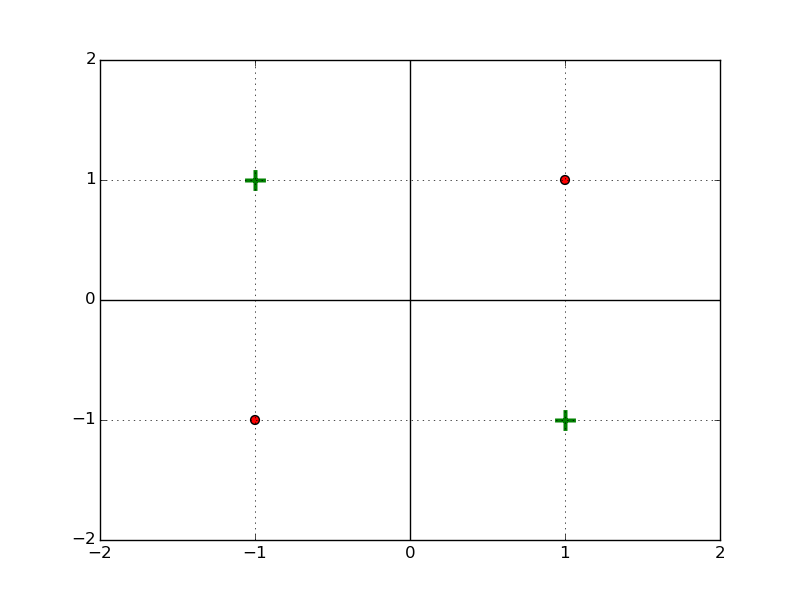
\includegraphics[width=3.3in]{plots/3C.png}
    \end{center}
    \end{figure}

\subproblem[5] Suppose we train a decision tree on this dataset using top-down greedy induction, with the Gini index as
the impurity measure. We define our stopping condition to be if no split of a node
results in any reduction in impurity. Submit a drawing of the resulting tree.  What is its classification error ((number of misclassified points) / (number of total points))?

\subproblem[5] Submit a drawing of a two-level decision tree that classifies the above dataset with zero classification error.  (You don't need to use any particular training algorithm to produce the tree.)

Is there any impurity measure (i.e. any function that maps the data points under a particular node in a tree to a real number) that would have led top-down greedy induction with the same stopping condition to produce the tree you drew?  If so, give an example of one, and briefly describe its pros and cons as an impurity measure for training decision trees in general (on arbitrary datasets). 

\subproblem[5] Suppose there are 100 data points in some 2-D dataset. What is the largest number of unique thresholds (i.e., internal nodes) you might need in order to achieve zero classification training error (on the training set)? Please
justify your answer.

\begin{solution}
$i.$ The tree is a stump with just a root node. The total impurity is 2 and the classification error is 0.5.

$ii.$ Any tree that splits on $x$ and $y$ (in either order) with proper leaf classifications works.
        
        There are infinite suitable impurity measures one could make up that would achieve this, but they all suffer various disadvantages (the main one being that they usually are dependent on the raw number of classified points under the leaf, which makes them bad for datasets of arbitrary size.)  As long as the student gives a function that works and explains why it's bad, they get credit.

    $iii$. If we have two identical data points, with different classifications, we can never achieve zero classification training error. So, we assume the data contains no identical points with different classifications. Then, we require at most 99 unique thresholds to classify the data. Consider, for
example, $S = \{(n, (-1)^n) | n \in \mathbb{N}, 1 \leq n \leq 100\}$. That is, we have points along one dimension, alternately classified as $-1, 1, -1, 1,-1, \hdots, 1$ Then, there is no
way to classify the points with fewer than 99 different thresholds.

    To show 99 unique thresholds is an upper-bound, we prove by construction that every set of 100 data points can be correctly classified with 100 unique thresholds. Order the data points in alphabetical order, that is initially by the first coordinate, then by the second coordinate, and so on. Now, beginning with $i= 1$, we add the $i$'th node to the tree such that the $i$'th sorted data point is correctly classified, by making the splitting criterion of the form $x_j(k) = y$, for $k$ the smallest coordinate which has not yet been split in the subtree. Note, this $i$'th split will also not affect the classifications of any $j$'th poin, for $j<i$, due to the sorting of the data points. After 100 steps, we have classified all 100 points correctly.
\end{solution}

\problem[4] Suppose in top-down greedy induction we want to split a leaf node that contains N data points composed of
D continuous features. What is the worst-case
complexity (big-O in terms of N and D) of the number of possible splits we must consider in order to find the one that most reduces impurity? Please justify your answer.

Note: Recall that at each node-splitting step in training a DT, you must consider all possible splits that you can make. While there are an infinite number of possible decision boundaries since we are using continuous features, there are not an infinite number of boundaries that result in unique child sets (which is what we mean by ``split'').



\begin{solution}
    At most, we must consider a split for each feature, for which there can be $N+1$ unique split points. Therefore, in the worst-case, we must consider $(N+1) \cdot D = O(ND)$ possible splits.
\end{solution}




\newpage


\section{Overfitting Decision Trees [30 Points]}
\materials{Lecture 5}

In this problem, you will use the Diabetic Retinopathy Debrecen Data Set, which contains features extracted from images to determine whether or not the images contain signs of diabetic retinopathy. Additional information about this dataset can be found at the link below:

\url{https://archive.ics.uci.edu/ml/datasets/Diabetic+Retinopathy+Debrecen+Data+Set}

In the following question, your goal is to predict the diagnosis of diabetic retinopathy, which is the final column in the data matrix.  Use the first 900 rows as training data, and the last
251 rows as validation data. Please feel free to use additional packages such as Scikit-Learn. Include your code in your submission.

\indent\problem[7] % indent for consistency
Train a decision tree classifier using Gini as the impurity measure and minimal leaf node size as early stopping criterion. Try different minimal leaf node sizes from 1 to 25 in increments of 1. Then, on a single plot, plot both training and test classification error versus leaf node size. To do this, fill in the \texttt{classification_err} and \texttt{eval_tree_based_model_min_samples} functions in the code template for this problem.

\begin{solution}
Please see the solution code, where we generate the following plot:
    \begin{figure}[H]
    \begin{center}
    \includegraphics[width=3.3in]{plots/fig2a.png}
    \caption{Decision Tree with Gini impurity and minimum node size as early-stopping criterion.}
    \end{center}
    \end{figure}
\end{solution}

\problem[7]
Train a decision tree classifier using Gini as the impurity measure and maximal tree depth as early stopping criterion. Try different tree depths from 2 to 20 in increments of 1. Then, on a single plot, plot both training and test classification error versus tree depth. To do this, fill in the \texttt{eval_tree_based_model_max_depth} function in the code template for this problem.

\begin{solution}
    We obtain the following plot:
    \begin{figure}[H]
    \begin{center}
    \includegraphics[width=3.3in]{plots/fig2b.png}
    \caption{Decision Tree with Gini impurity and minimum node size as early-stopping criterion.}
    \end{center}
    \end{figure}
\end{solution}

\problem[4]
For both the minimal leaf node size and maximum depth parameters tested in the last two questions, which parameter value minimizes the test error? What effects does early stopping have on the performance of a decision tree model?
Please justify your answer based on the two plots you derived.

\begin{solution}
    Early stopping will improve testing error. Using the Minimum Node Size stopping criterion, we see minimum testing error is reached at minimum node size 12. Likewise, using the Maximum Tree Depth stopping criterion, we see minimum testing error is reached at maximum tree depth of 2. Both are improvements over cases without early stopping (1 minimum node size, 20 maximum tree depth). In both cases, therefore, early stopping improves testing error. (The locations of the minima can vary slightly between runs, but using the random seed of 1 that we provided in the template, one should get these values.)
\end{solution}

\indent\problem[2] % indent for consistency
Train a random forest classifier using Gini as the impurity measure, minimal leaf node size as early stopping criterion, and 1,000 trees in the forest. Try different node sizes from 1 to 25 in increments of 1. Then, on a single plot, plot both training and test classification error versus
leaf node size.

\begin{solution}
    We obtain the following plot:
    \begin{figure}[H]
    \begin{center}
    \includegraphics[width=3.3in]{plots/fig2d.png}
    \caption{Random forest with Gini impurity and minimum node size as early-stopping criterion.}
    \end{center}
    \end{figure}
\end{solution}

\problem[2]
Train a random forest classifier using Gini as the impurity measure, maximal tree depth as early stopping criterion, and 1,000 trees in the forest. Try different tree depths from 2 to 20 in increments of 1. Then, on a single plot, plot both training and test classification error versus tree depth.

\begin{solution}
    We obtain the following plot:
    \begin{figure}[H]
    \begin{center}
    \includegraphics[width=3.3in]{plots/fig2e.png}
    \caption{Random forest with Gini impurity and minimum node size as early-stopping criterion.}
    \end{center}
    \end{figure}
\end{solution}

\problem[4]
For both the minimal leaf node size and maximum depth parameters tested, which parameter value minimizes the random forest test error? What effects does early stopping have on the performance of a random forest model?
Please justify your answer based on the two plots you derived.

\begin{solution}
 Early stopping makes the test error worse. Using the Minimum Node Size stopping criterion, we see minimum testing error is reached at minimum node size of 1. Likewise, using the Maximum Tree Depth stopping criterion, we see minimum testing error is reached at maximum tree depth of 12.  (The locations of the minima can vary slightly between runs, but using the random seed of 1 that we provided in the template, one should get these values.)
\end{solution}

\problem[4]
Do you observe any differences between the curves for the random forest and decision tree plots? If so, explain what could account for these differences.

\begin{solution}
Random forests give somewhat smoother curves than decision trees, because they average over a large number of decision trees. One can also see from the plots that the random forests tend to achieve lower errors on the test set than the decision trees. Additionally, we see that with both types of stopping conditions, the test error is optimized for deeper trees, whereas with decision trees, the optimal stopping conditions favored shallower trees. This is because decision trees are highly-prone to overfitting, while random forests average over a large number of trees, thereby decreasing model variance. 
\end{solution}



\newpage
\section{The AdaBoost Algorithm [40 points]}
\materials{Lecture 6}

In this problem, you will show that the choice of the $\alpha_t$ parameter in
the AdaBoost algorithm corresponds to greedily minimizing an exponential upper
bound on the loss term at each iteration.

\problem[3]
Let $h_t: \mathbb{R}^m \rightarrow \{-1,1\}$ be the weak classifier obtained at step $t$, and let $\alpha_t$ be
its weight. Recall that the final classifier is $$H(x) = \text{sign}(f(x)) = \text{sign} \left(\sum\limits_{i=1}^T \alpha_{t}h_t(x) \right).$$

Suppose $\{(x_1, y_1), ..., (x_N, y_N)\} \subset \mathbb{R}^m \times \{-1,1\}$ is our training dataset.  Show that the training set error of the final classifier can be bounded from
above if an an exponential loss function is used:

$$E = \frac{1}{N} \sum\limits_{i=1}^N \exp(-y_{i}f(x_i)) \geq \frac{1}{N} \sum\limits_{i=1}^N \mathbbm{1}(H(x_i) \neq y_i),$$

where $\mathbbm{1}$ is the indicator function.

\begin{solution}
	The inequality is true if each term satisfies the inequality. So, we show 
	\[ 
	\exp(-y_i f(x_i)) \geq \mathbbm{1}(H(x_i) \neq y_i).
	\]
	First, consider any points correctly classified. This means $H(x_i) = y_i \implies \mathbbm{1}(H(x_i) \neq y_i) = 0.$ Then, since $e^x \geq  0 \ \forall x$, we have
	\[
	\exp(-y_i f(x_i)) \geq 0 = \mathbbm{1}(H(x_i) \neq y_i).
	\]
	Next, consider any points incorrectly classified. This means $H(x_i) \neq y_i \implies \mathbbm{1}(H(x_i) \neq y_i) = 1.$ Then, note for incorrectly classified points, $\text{sign}(f(x_i)) \neq y_i \implies -y_i f(x_i) \geq 0$ Then, since $e^x \geq 1 \ \forall x \geq 0$, we have
	\[
	\exp(-y_i f(x_i)) \geq 1 = \mathbbm{1}(H(x_i) \neq y_i).
	\]
	
	Thus, every term in the sequence corresponding to a correctly or incorrectly classified point is bounded above by the exponential loss function $E$. Therefore,
	\[
	\boxed{E = \frac{1}{N}\sum_{i=1}^N \exp(-y_i f(x_i)) \geq \frac{1}{N} \sum_{i=1}^N
		\mathbbm{1}(H(x_i) \neq y_i)}.
	\]
\end{solution}

\problem[3]
Find $D_{T + 1}(i)$ in terms of $Z_t$, $\alpha_t$, $x_i$, $y_i$, and the classifier $h_t$, where $T$ is the last timestep and $t \in \{1, \ldots, T\}$. Recall that $Z_t$ is the normalization factor for distribution $D_{t+1}$:
$$Z_t = \sum\limits_{i=1}^N D_t(i) \exp(-\alpha_{t}y_{i}h_{t}(x_{i})).$$

\begin{solution}
	We note
	\[
	D_1(i) = \frac{1}{N} \tag{1}
	\] and
	\[
	D_{t+1}(i) = \frac{D_t(i)\exp(-\alpha_t y_i h_t(x_i))}{Z_t}, \tag{2}
	\] where $Z_t$ is a normalization factor chosen so that $D_{t+1}$ will be a distribution. That is,
	\[
	Z_t = \sum_{i=1}^N D_t(i) \exp(-\alpha_t y_i h_t(x_i)). 
	\]
	\par
	Using (1) and (2), we find
	\[
	\boxed{D_{T+1}(i) = \frac{1}{N} \prod_{t=1}^T\frac{e^{-\alpha_t y_i h_t(x_i)}}{Z_t}}.
	\]
\end{solution}

\problem[2]
Show that $E = \sum_{i=1}^N  \frac{1}{N} e^{\sum_{t=1}^T -\alpha_t y_i h_t(x_i)}.$

\begin{solution}
	Recall that \[E = \frac 1 N \sum_{i = 1}^N e^{- y_i f(x_i)}.\]
	Note that \[f(x_i) = \sum_{t = 1}^T \alpha_t h_t(x_i).\]
	So \[\boxed{E = \sum_{i=1}^N  \frac{1}{N} e^{\sum_{t=1}^T -\alpha_t y_i h_t(x_i)}}.\]
\end{solution}

\problem[5]
Show that
$$E = \prod\limits_{t=1}^T Z_t.$$

\begin{hint}
	Recall that $\sum_{i = 1}^N D_t(i) = 1$ because $D$ is a distribution.
\end{hint}

\begin{solution}
	We found above that 
	\[
	D_{T+1}(i) = \frac{1}{N} \prod_{t=1}^T\frac{e^{-\alpha_t y_i h_t(x_i)}}{Z_t}.
	\]
	
	This implies
	\[
	D_{T+1}(i) \cdot \prod_{t=1}^T {Z_t} = \frac{1}{N} \prod_{t=1}^T e^{-\alpha_t y_i h_t(x_i)}
	\]
	\[
	\implies D_{T+1}(i) \cdot \prod_{t=1}^T {Z_t} =  \frac{1}{N} e^{\sum_{t=1}^T -\alpha_t y_i h_t(x_i)}
	\]
	\[
	\implies \sum_{i=1}^N  D_{T+1}(i) \cdot \prod_{t=1}^T {Z_t} = \sum_{i=1}^N  \frac{1}{N} e^{\sum_{t=1}^T -\alpha_t y_i h_t(x_i)}
	\]
	\[
	\implies \sum_{i=1}^N D_{T+1}(i) \prod_{t=1}^T {Z_t} = \sum_{i=1}^N  \frac{1}{N} e^{\sum_{t=1}^T -\alpha_t y_i h_t(x_i)}.
	\]
	We showed above that the right side is equal to $E$.  We also know that $\sum_{i=1}^N D_{T+1}(i) = 1$ as in the hint.
	\[
	\implies \boxed{\prod_{t=1}^T {Z_t} =E}.
	\]
\end{solution}

\problem[5]
Show that the normalizer $Z_t$ can be written as
\[Z_t = (1 - \epsilon_t) \exp(-\alpha_t) + \epsilon_{t} \exp(\alpha_t)\]
where $\epsilon_t$ is the training set error of weak classifier $h_t$ for the weighted dataset:
\[\epsilon_t = \sum\limits_{i=1}^N D_t(i)\mathbbm1(h_t(x_i) \neq y_i).\]

\begin{solution}
	Note, 
	\[
	Z_t = \sum_{i=1}^N D_t(i) \exp(-\alpha_t y_i h_t(x_i)).
	\]
	Note, if $h_t$ classifies point $x_i$ correctly (so $h_t(x_i) * y_i = 1$), we have
	\[ D_t(i) \exp(-\alpha_t y_i h_t(x_i)) = D_t(i) \exp(-\alpha_t) = (1  - \mathbbm{1}(h_t(x_i) \neq y_i))D_t(i) \exp(-\alpha_t). \] Note, if $h_t$ classifies point $x_i$ incorrectly (so $h_t(x_i) * y_i = -1$), we have 
	\[ D_t(i) \exp(-\alpha_t y_i h_t(x_i)) = D_t(i) \exp(\alpha_t) = \mathbbm{1}(h_t(x_i) \neq y_i) D_t(i) \exp(\alpha_t).\]
	So \[Z_t = \sum_{i=1}^N D_t(i) \exp(-\alpha_t y_i h_t(x_i))\]
	\[ \implies Z_t =  \sum_{i=1}^N (1  - \mathbbm{1}(h_t(x_i) \neq y_i))D_t(i) \exp(-\alpha_t) + \mathbbm{1}(h_t(x_i) \neq y_i) D_t(i) \exp(\alpha_t)) \]
	\[ = \left(\sum_{i=1}^N D_t(i) - \sum_{i = 1}^N \mathbbm{1}(h_t(x_i) \neq y_i)D_t(i)\right)\exp(-\alpha_t) + \sum_{i = 1}^N\mathbbm{1}(h_t(x_i) \neq y_i) D_t(i) \exp(\alpha_t) = \]
	\[\implies \boxed{Z_t = (1-\epsilon_t)\exp(-\alpha_t) + \epsilon_t \exp(\alpha_t)}\]
	because $\sum_{i=1}^N D_t(i) = 1$.
	
\end{solution}

\problem[2]
We derived all of this because it is hard to directly minimize the training set error, but we can greedily minimize the upper bound $E$ on this error. Show that choosing $\alpha_t$
greedily to minimize $Z_t$ at each iteration leads to the choices in
AdaBoost:
$$\alpha_{t}^* = \frac{1}{2} \ln \left(\frac{1 - \epsilon_t}{\epsilon_t} \right).$$

\begin{solution}
	\[Z_t = (1-\epsilon_t)\exp(-\alpha_t) + \epsilon_t \exp(\alpha_t)\]
	
	We note $Z_t$ is convex, so to minimize $Z_t$, we find $\alpha_t$ such that  
	\[
	\frac{dZ_t}{d \alpha_t} = -(1-\epsilon_t)\exp(-\alpha_t) + \epsilon_t \exp(\alpha_t) = 0
	\]
	Multiplying by $\exp(\alpha_t)$,
	\[
	\implies -(1-\epsilon_t) + \epsilon_t \exp(2\alpha_t) = 0.
	\]
	\[
	\implies  \epsilon_t \exp(2\alpha_t) = 1-\epsilon_t
	\]
	\[
	\implies  \exp(2\alpha_t) = \frac{1-\epsilon_t}{\epsilon_t }
	\]
	\[
	\implies  \boxed{\alpha_t = \frac{1}{2} \ln \left( \frac{1-\epsilon_t}{\epsilon_t } \right)}.
	\]
	
\end{solution}

\begin{problem}[14]
    Implement the \texttt{GradientBoosting.fit()} and \texttt{AdaBoost.fit()} methods in the notebook provided for you. Some important notes and guidelines follow:
    \begin{itemize}
        \item For both methods, make sure to work with the class attributes provided to you. Namely, after \texttt{GradientBoosting.fit()} is called, \texttt{self.clfs} should be appropriately filled with the \texttt{self.n_clfs} trained weak hypotheses. Similarly, after \texttt{AdaBoost.fit()} is called, \texttt{self.clfs} and \texttt{self.coefs} should be appropriately filled with the \texttt{self.n_clfs} trained weak hypotheses and their coefficients, respectively.
        \item \texttt{AdaBoost.fit()} should additionally return an $(N, T)$ shaped numpy array \texttt{D} such that \texttt{D[:, t]} contains $D_{t+1}$ for each $t \in \{0, \ldots, \texttt{self.n_clfs}\}$.
        \item For the \texttt{AdaBoost.fit()} method, \textbf{use the 0/1 loss} instead of the exponential loss.
	\item The only Sklearn classes that you may use in implementing your boosting fit functions are the DecisionTreeRegressor and DecisionTreeClassifier, not GradientBoostingRegressor.
    \end{itemize}
\end{problem}

\begin{problem}[2]
    Describe and explain the behaviour of the loss curves for gradient boosting and for AdaBoost. You should consider two kinds of behaviours: the smoothness of the curves and the final values that the curves approach.
\end{problem}
\begin{solution}
    Training loss in gradient boosting decreases in a smooth fashion towards 0, but test loss stops decreasing quickly and then flattens with a slight increase. Training and test losses in AdaBoost both steadily approach relatively-small values without increasing much, and are not smooth (lots of spikes). This is attributed to the fact that AdaBoost uses classifiers, not regressors.
\end{solution}

\begin{problem}[2]
    Compare the final loss values of the two models. Which performed better on the classification dataset?
\end{problem}
\begin{solution}
    Gradient boosting performed better on training but AdaBoost performed better on test. That is, AdaBoost performed better overall as it is naturally more inclined to a classification dataset (it uses classifiers as opposed to regressors).
\end{solution}

\begin{problem}[2]
    For AdaBoost, where are the dataset weights the largest, and where are they the smallest?
\end{problem}
\begin{hint}
    Watch how the dataset weights change across time in the animation.
\end{hint}
\begin{solution}
    The weights are the largest where there is the most ambiguity in classes. In the case of the given dataset, they are largest at the the edges of the spirals and smallest away from these edges.
\end{solution}

\newpage
\section{Convex Functions [7 points, EC 3 Points]}

\emph{This problem further develops the ideas of convex functions, and provides intuition for why convex optimization is so important for
 Machine Learning.}

Given a convex set $\mathcal{X}$, a function $f:\mathcal{X}\to\mathbb{R}$ is \textbf{convex} if for all $\textbf{x},\textbf{y}\in \mathcal{X}$ and all $t\in[0,1]$ :
\[f(t\textbf{x} + (1-t)\textbf{y}) \leq tf(\textbf{x}) + (1-t)f(\textbf{y})\]

\begin{problem}[3]
Let $\mathcal{X}$ be a convex set. If $f$ is a convex function, show that any local minimum of $f$ in $\mathcal{X}$ is also a global minimum.
\end{problem}

\begin{solution}
\begin{proof}
Let $\textbf{x}^*$ be a local minimum of $f$ in $\mathcal{X}$. Then, for some neighborhood $\mathrm N\subseteq \mathcal{X}$ around $\mathbf{x}^*$, we have that $f(\mathbf{x})\geq f(\mathbf{x}^*)$, for all $x\in \mathrm N$. Assume (by way of contradiction) that there exists $\tilde{\mathbf{x}} \in \mathcal{X}$ such that $f(\tilde{\mathbf{x}}) < f(\mathbf{x}^*)$.\\

Then, consider the line segment $\mathbf{x}(t) = t\mathbf{x}^* + (1-t)\tilde{\mathbf{x}}$, for $t\in [0,1]$, where we note that $\mathbf{x}(t)\in \mathcal{X}$ by the convexity of $\mathcal{X}$. Then, by the convexity of $f$, we see that for all $t\in(0,1)$: 
\[f(\mathbf{x}(t)) \leq tf(\mathbf{x}^*) + (1-t)f(\tilde{\mathbf{x}}) < tf(\mathbf{x}^*) + (1-t)f(\mathbf{x}^*) = f(x^*)\]
We can pick $t$ to be sufficiently close to $1$ that $\mathbf{x}(t) \in \mathrm N$. Then, $f(\mathbf{x}(t)) \geq f(\mathbf{x}^*)$ by the definition of $\mathrm N$, but the above inequality states that $f(\mathbf{x}(t)) < f(\mathbf{x})$, which is a contradiction. \\

Therefore, $f(\mathbf{x}^*) < f(\mathbf{x})$ for all $\mathbf{x}\in\mathcal{X}$, so $\mathbf{x}^*$ is a global minimum of $f$ in $\mathcal{X}$. \qedhere
\end{proof}
\end{solution}

\begin{problem}[4]
\emph{Using part A}, explain why convex loss functions are desirable when training learning models.
\end{problem}

\begin{solution}
There are many possible answers here:\\
1) Most intuitive algorithms work: any form of gradient descent (just going down the loss function) leads you to the local minimum which is also the global minimum. \\
2) Cannot get stuck at a local minima.\\
3) The optimal solution is absolutely computable, and the computational solution will equal the theoretical optimum.
\end{solution}

\problem\textbf{[3 points, Extra Credit] }
The Kullback-Leibler (KL) divergence is a measure of statistical distance between two probability distributions $(p, q)$, also called the relative entropy. KL divergence can be used to generate optimal parameters for visualization models (which we will also see in set 4).
\[\mathrm{KL}[P\|Q] = \sum_{x\in\mathcal{X}} p(x) \cdot \log \frac{p(x)}{q(x)}\]
Show that the KL divergence is a convex loss function. \\

\begin{hint}
    Use the log sum inequality
\end{hint}

\begin{solution}
\begin{proof}
The log sum inequality states that for non-negative real numbers $a_1, \dots, a_n, b_1, b_n$, that:
\[\sum_{i=1}^n a_i \log \frac{a_i}{b_i} \geq \left(\sum_{i=1}^n a_i\right)\log \frac{\sum_{i=1}^n a_i}{\sum_{i=1}^n b_i}\]
 Then, observe that:
 \begin{align*}
     &\mathrm{KL}[\lambda p_1 + (1-\lambda)p_2 \| \lambda q_1 + (1-\lambda)q_2] \\
     &= \sum_{x\in \mathcal{X}} \left[[\lambda p_1(x) + (1-\lambda) p_2(x)] \cdot \log \frac{\lambda p_1 (x) + (1-\lambda) p_2 (x)}{\lambda q-1 (x) + (1-\lambda) q_2(x)}\right] \\
     &\leq \sum_{x\in \mathcal{X}} \left[\lambda p_1(x) \cdot \log \frac{\lambda p_1(x)}{\lambda q_1 (x)}+ (1-\lambda) p_2(x) \cdot \log \frac{(1-\lambda) p_2 (x)}{(1-\lambda) q_2(x)}\right] \\
     &= \lambda \sum_{x\in \mathcal{X}} p_1(x) \cdot \log \frac{ p_1(x)}{q_1 (x)} + (1-\lambda)\sum_{x\in\mathcal{X}} p_2(x) \cdot \log \frac{p_2 (x)}{q_2(x)} \\
     &= \lambda \mathrm{KL}[p_1 \| q_1] + (1-\lambda)\mathrm{KL}[p_2 \| q_2]
 \end{align*}
 Therefore, since 
 \[\mathrm{KL}[\lambda p_1 + (1-\lambda)p_2 \| \lambda q_1 + (1-\lambda)q_2] = \lambda \mathrm{KL}[p_1 \| q_1] + (1-\lambda)\mathrm{KL}[p_2 \| q_2]\]
 we can conclude that the KL divergence is a convex function.
 \qedhere
\end{proof}
\end{solution}
\end{document}